\documentclass{beamer}
\usepackage[utf8]{inputenc}

\usetheme{Madrid}
\usecolortheme{default}
\usepackage{amsmath,amssymb,amsfonts,amsthm}
\usepackage{mathtools}
\usepackage{txfonts}
\usepackage{tkz-euclide}
\usepackage{listings}
\usepackage{adjustbox}
\usepackage{array}
\usepackage{gensymb}
\usepackage{tabularx}
\usepackage{gvv}
\usepackage{lmodern}
\usepackage{circuitikz}
\usepackage{tikz}
\lstset{literate={·}{{$\cdot$}}1 {λ}{{$\lambda$}}1 {→}{{$\to$}}1}
\usepackage{graphicx}
\usepackage{multicol}

\setbeamertemplate{page number in head/foot}[totalframenumber]

\usepackage{tcolorbox}
\tcbuselibrary{minted,breakable,xparse,skins}



\definecolor{bg}{gray}{0.95}
\DeclareTCBListing{mintedbox}{O{}m!O{}}{%
  breakable=true,
  listing engine=minted,
  listing only,
  minted language=#2,
  minted style=default,
  minted options={%
    linenos,
    gobble=0,
    breaklines=true,
    breakafter=,,
    fontsize=\small,
    numbersep=8pt,
    #1},
  boxsep=0pt,
  left skip=0pt,
  right skip=0pt,
  left=25pt,
  right=0pt,
  top=3pt,
  bottom=3pt,
  arc=5pt,
  leftrule=0pt,
  rightrule=0pt,
  bottomrule=2pt,
  toprule=2pt,
  colback=bg,
  colframe=orange!70,
  enhanced,
  overlay={%
    \begin{tcbclipinterior}
    \fill[orange!20!white] (frame.south west) rectangle ([xshift=20pt]frame.north west);
    \end{tcbclipinterior}},
  #3,
}
\lstset{
    language=C,
    basicstyle=\ttfamily\small,
    keywordstyle=\color{blue},
    stringstyle=\color{orange},
    commentstyle=\color{green!60!black},
    numbers=left,
    numberstyle=\tiny\color{gray},
    breaklines=true,
    showstringspaces=false,
}
%------------------------------------------------------------
%This block of code defines the information to appear in the
%Title page
\title %optional
{2.10.45}
\date{October 1,2025}
%\subtitle{A short story}

\author % (optional)
{Taraka Abhinav - EE25BTECH11016}



\begin{document}


\frame{\titlepage}


\begin{frame}{Question}
If $\vec{a}$ and $\vec{b}$ are two unit vectors such that $\vec{a} + 2\vec{b}$ and $5\vec{a} - 4\vec{b}$ are perpendicular to each other, then the angle between $\vec{a}$ and $\vec{b}$ is:

\begin{enumerate}

    \item $45^\circ$
    \item $60^\circ$
    \item $\arccos \frac{1}{3}$
    \item $\arccos \frac{2}{7}$
\end{enumerate}
\end{frame}

\begin{frame}{Step 1: The Perpendicularity Condition}
The vectors are perpendicular, so their dot product is zero. In matrix notation:
\begin{align}
    (\vec{a} + 2\vec{b})^T (5\vec{a} - 4\vec{b}) = 0 \label{eq:perp_condition}
\end{align}
Expanding this expression:
\begin{align}
    (\vec{a}^T + 2\vec{b}^T) (5\vec{a} - 4\vec{b}) &= 0 \nonumber \\
    5(\vec{a}^T\vec{a}) - 4(\vec{a}^T\vec{b}) + 10(\vec{b}^T\vec{a}) - 8(\vec{b}^T\vec{b}) &= 0 \label{eq:expanded}
\end{align}
\end{frame}

\begin{frame}{Step 2: Simplifying with Vector Properties}
Since $\vec{a}^T\vec{b} = \vec{b}^T\vec{a}$ (dot product is commutative), we get:
\begin{align}
    5(\vec{a}^T\vec{a}) + 6(\vec{a}^T\vec{b}) - 8(\vec{b}^T\vec{b}) = 0 \label{eq:simplified}
\end{align}
The vectors are unit vectors, so their squared magnitude is 1:
\begin{align}
    \vec{a}^T\vec{a} = 1 \quad \text{and} \quad \vec{b}^T\vec{b} = 1 \label{eq:unit_vectors}
\end{align}
Substituting this into equation \eqref{eq:simplified}:
\begin{align}
    5(1) + 6(\vec{a}^T\vec{b}) - 8(1) = 0 \implies \vec{a}^T\vec{b} = \frac{1}{2} \label{eq:dot_product_value}
\end{align}
\end{frame}

\begin{frame}{Step 3: Finding the Angle}
The angle $\theta$ is defined by $\vec{a}^T\vec{b} = |\vec{a}||\vec{b}|\cos\theta$.
\begin{align}
    \cos\theta = \frac{\vec{a}^T\vec{b}}{|\vec{a}||\vec{b}|} = \frac{1/2}{(1)(1)} = \frac{1}{2}
\end{align}
Therefore, the angle is:
\[ \theta = \arccos\left(\frac{1}{2}\right) = 60^\circ \]
The correct option is (b).
\end{frame}

\begin{frame}[fragile]
    \frametitle{C Code - Verification}
    \begin{lstlisting}
#include <stdio.h>
#include <math.h>

// Function to compute angle between two vectors
double find_angle(double a[2], double b[2]) {
    double dot = a[0]*b[0] + a[1]*b[1];
    double mag_a = sqrt(a[0]*a[0] + a[1]*a[1]);
    double mag_b = sqrt(b[0]*b[0] + b[1]*b[1]);
    return acos(dot / (mag_a * mag_b));
}

int main() {
    // Unit vectors with 60 deg between them
    double a[2] = {1, 0};
    double b[2] = {0.5, sqrt(3)/2};

    double theta = find_angle(a,b);
    printf("Angle = %.2f deg\n", theta*180/M_PI);
    return 0;
}
    \end{lstlisting}
\end{frame}

\begin{frame}[fragile]
    \frametitle{Python + C Code}
    \begin{lstlisting}[language=Python]
import ctypes
import numpy as np

# Load C shared library
# Compile with: gcc -shared -o angle_vectors.so -fPIC angle.c -lm
lib = ctypes.CDLL("./angle_vectors.so")

# Define argtypes and restype
lib.find_angle.argtypes = [ctypes.POINTER(ctypes.c_double),
                           ctypes.POINTER(ctypes.c_double)]
lib.find_angle.restype = ctypes.c_double

# Define vectors
a = (ctypes.c_double * 2)(1, 0)
b = (ctypes.c_double * 2)(0.5, np.sqrt(3)/2)

# Call C function
theta = lib.find_angle(a, b) * 180 / np.pi
print(f"Angle between vectors = {theta:.2f} degrees")
    \end{lstlisting}
\end{frame}

\begin{frame}[fragile]
    \frametitle{Pure Python Code}
    \begin{lstlisting}[language=Python]
import numpy as np
import matplotlib.pyplot as plt

# Define unit vectors
A = np.array([1, 0])
B = np.array([0.5, np.sqrt(3)/2])

# Compute angle
dot = np.dot(A, B)
norm_prod = np.linalg.norm(A) * np.linalg.norm(B)
theta = np.degrees(np.arccos(dot / norm_prod))
print(f"Angle between vectors = {theta:.2f} degrees")
    \end{lstlisting}
\end{frame}

\begin{frame}[fragile]
    \frametitle{Python Plotting Code}
    \begin{lstlisting}[language=Python]
# Plot vectors
O = np.array([0,0])
plt.quiver(*O, A[0], A[1], angles='xy', scale_units='xy', scale=1, color='r', label='a')
plt.quiver(*O, B[0], B[1], angles='xy', scale_units='xy', scale=1, color='b', label='b')

# Display angle
plt.text(0.2, 0.1, f"{theta:.2f}°", fontsize=12, color='purple')

plt.xlim(-0.2, 1.2); plt.ylim(-0.2, 1.2)
plt.grid(True); plt.gca().set_aspect('equal')
plt.title("Unit Vectors with 60° Angle")
plt.legend(); plt.savefig("figs/Figure_1.png")
plt.show()
    \end{lstlisting}
\end{frame}

\begin{frame}{Plot}
    \frametitle{Plot of the Unit Vectors}
    \centering
    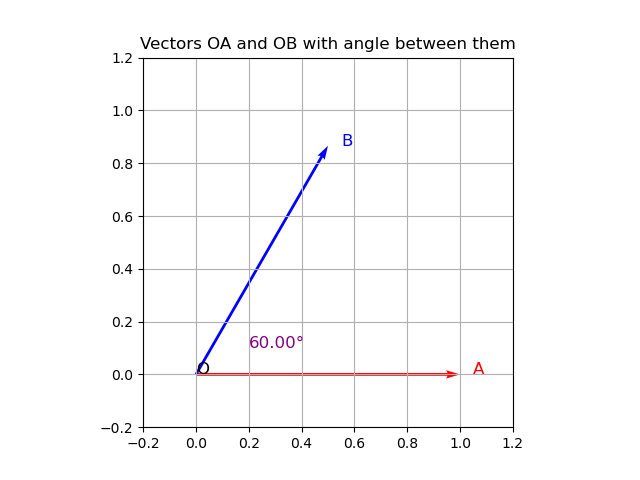
\includegraphics[width=0.7\textwidth]{figs/Figure_1.png}   
\end{frame}

\end{document}